\documentclass [a4paper,final,conference,10pt]{IDAACS}
\usepackage[utf8]{inputenc}
\usepackage[english]{babel}
\usepackage{amsmath}
\usepackage{graphicx}
\usepackage{multirow}
\usepackage{cite}
\usepackage{pgfplots}
\usepackage{pgfplotstable}
%\title{Effective Parallelization of Mixed-Critical Software to Distributed Heterogeneous Mutlicoresystems}
%\subtitle{
%	Approaching Challenges of Automotive Constrains: Partial Realtime, Safety, Affinity and Connectivity}
%Bare-Metal and OS-based 
%\title{Constrained Parallelization of Mixed-Critical Applications to Distributed Heterogeneous Hardware}
\title{Constrained Mixed-Critical Parallelization for Distributed Heterogeneous Systems}
\author{
\IEEEauthorblockN{Robert Höttger, Mustafa Özcelikörs, Lukas Krawczyk, Philipp Heisig, Carsten Wolff, Burkhard Igel}
%						Third Author's Name\IEEEauthorrefmark{2}}
\IEEEauthorblockA{Dortmund University of Applied Sciences and Arts - IDiAL Institute, \\\{robert.hoettger, mustafa.ozcelikors, lukas.krawczyk,  philipp.heisig, carsten.wolff, igel\}@fh-dortmund.de \\ www.idial.institute 
%						\IEEEauthorrefmark{2}Affiliation, Postal address, e-mail, Web address (URL)\\
%						\IEEEauthorrefmark{3}Affiliation, Postal address, e-mail, Web address (URL)\\
	}
}
\begin{document}
\maketitle

\let\thefootnote\relax\footnotetext{As part of the AMALTHEA4public project, this work has been funded by the German Federal Ministry of Education and Research - BMBF, under funding no. $01|S14029K$}

\begin{abstract}
Distributing software effectively to multi-core, many-core, and distributed systems has been studied for decades and still advances successively driven by domain specific constraints. Programming vehicle ECUs (Electronic Constrol Units) is one of the most constrained domains that just recently approached the need for concurrency due to advanced driver assistant systems or autonomous driving approaches. In this paper, various challenges for such systems are outlined, discussed, and solutions are given upon instruction precise modeling, affinity constrained based distribution, and effective software parallelization. The solutions are compared upon bare-metal and OS based implementations while considering fixed priorities for sequential, OS based, and APP4MC scheduling. The latter case has been published at \cite{ICPDSSE} and evolved to consider affinity constraints, SWC-based partitioning and communication cost related mapping. Results show that using APP4MC based distributions on a distributed heterogeneous system outperforms available approaches for mixed-critical applications.
%TODO percent
\end{abstract}

\begin{IEEEkeywords}
Constrained parallelization, heterogeneous systems, distributed systems, multicore, parallel embedded systems
\end{IEEEkeywords}

\section{Introduction}
Especially the automotive domain requires lots of constraints originating from different safety, security, timing, or similar requirements. The verification, validation, testing, and simulation stack requires dozens of tools and the consideration of established architectures, standards, models, and assessments to address product-line supporting, consistent, modular, and scalable software. However, these efforts lack in transparency likewise the comprehensive understanding of applications. Recent approaches such as APP4MC\footnote{\underline{APP}lication \underline{P}latform \underline{P}roject for Multi and Manycore, http://eclip.se/a7, access February 2017} already address this challenge and try to provide a common adaptable platform based on AUTOSAR while providing a standardized data model. Any specific commercial or proprietary tooling is supposed to be integratable in order to provide seamless interaction with provided tooling such as product-line management, requirements engineering, partitioning, mapping, testing, and more. 

In this paper, use the open source APP4MC environment in order to address both industrial and research related models while evaluating our new developments not only regarding model results but also to validate result among a specific use case described in section \ref{sec:rccar}. The RC-Car is an advanced demonstrator that features 16 100MHz logical cores (XMOS ExplorerKit, XCore-200) 
%2 instructions per cycle see https://www.xmos.com/download/private/xCORE-Architecture-Flyer%281.1%29.pdf
%2000MIPS 16 core https://www.xmos.com/download/private/xCORE-200-XE-Product-Brief%281.2%29.pdf
%--> 125MIPS per logical core, --> 1,25 instructions per cycle?
combined with four cores clocked at 1200MHz (Raspberry Pi 3, ARM CoreTex-A53).

The further remainder of this paper is structured as follows: The next section \ref{sec:app4mc} describes roughly the environment this contribution is based upon. Afterwards, section \ref{sec:rccar} illustrates capabilities and properties of the RC-Car demonstrator. Subsequently, section \ref{sec:impl} outlines the specific developments and solutions to precise modeling and software parallelization that is evaluated and compared to related approaches in section \ref{sec:eval}. Finally, section \ref{sec:concl} concludes this paper's contributions and discusses benefits, disadvantages, possible extensions, and promising outlooks that potentially advance the current approach.

\section{APP4MC}
\label{sec:app4mc}
TEst
%FOCUS Constraints
APP4MC is an open source project for developing multi and many core systems primarily for the automotive domain. Instead of describing its different purposes and features, the focus of this section concentrates on the required steps to utilize APP4MC parallelization capabilities \cite{ICPDSSE} i.e. partitioning and mapping. Those processes have been advanced in recent years to consider affinity, allocation, and safety constraints among others. Dealing with safety constraints ensures that tasks having a specific \underline{A}utomotive \underline{S}afety \underline{I}ntegrity \underline{L}evel (ASIL) are allocated to processing units (cores) featuring the corresponding ASIL level. Allocation constraints are considered the same way, except that instead of ASIL levels, properties such as \underline{F}loating \underline{P}oint \underline{U}nit (FPU) connectivity, cache memory size, processing frequency or others are investigated. Affinity constraints are evaluated within the partitioning process since runnables, i.e. smallest executable units, have to be kept in the same partition that are later on resolved to tasks. This paper's application, i.e. the RC-Car, features all of those constraints. Affinity has to be kept for instance regarding the light system state task and the \underline{P}ulse \underline{W}idth \underline{M}odulation (PWM) signal generation (timer) tasks since their distribution would cause implementation and communication overheads. Since there are tasks that continuously check the core utilization on each X-Core Tile, those tasks feature an allocation constraint to each X-Core Tile. Finally, due to the fact that the RC-Car performs image processing from a camera as well as real time tasks for motor control, steering and bluetooth based communications, we define all tasks that are crucial for safe driving as being safety critical (safety constraint) and bind them to the real time capable XMOS board. 

Apart from the constraints, software and hardware descriptions are required. While the hardware model is created manually, a C/CPP parser was used to receive necessary AMALTHEA software model data i.e. runnables, labels, label accesses, activations, runnable calls, \underline{I}nterrupts \underline{S}ervice \underline{R}outines (ISRs), Semaphores, and more for the Raspberry (RPI) implementations. Excerpts of those models are shown in Figure~\ref{fig:model}. While the RPI already features 247 Runnables and more, XMOS implementations were modeled on a higher level upon threads only, that correspond tasks. Those count 30 in total where profiling was performed via counting assembler instructions and using XXX for profiling.
%TODO insert how instructions of XMOS threads was found out
test
\begin{figure}[bth]
	\centering
	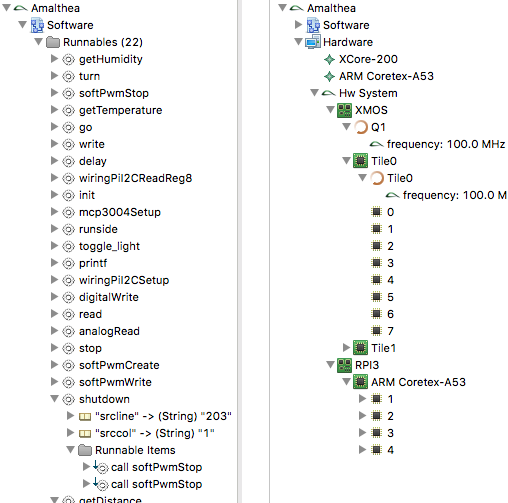
\includegraphics[scale=0.3]{images/models.png}
	\caption{\label{fig:model}AMALTHEA software and hardware models (excerpts) for the RC-Car}
\end{figure}
Before the partitioning and mapping processes can be configured and executed, one of the most challenging key property has to be added to runnables i.e. the above mentioned affinity, allocation, and safety constraints.
\section{RC-Car}
\label{sec:rccar}
The current Raspberry Pi distribution includes processes for the touchscreen, ethernet communication, core utilization reader, mjpg streamer, vnc application, apache2, OpenCV image processing, and additional cyclewaster. The latter processes can be added in order to push the core utilization to a maximum and consider high workload. The effective distribution provided by APP4MC is here crucial to provide deadline violation free program execution. 

The XMOS tasks focus on necessary real time implementations. Scheduling on the XMOS is non preemptive and allows a better determinism as well as easier WCET reasoning due to less context switching and less scheduling jitter \ref{xmos}. However, since our number of tasks exceed the total number of available cores on the XMOS, we had to define high priority tasks, that run on dedicated cores, and low priority tasks that run concurrently with other low level tasks in cooperative multitask manner on common cores. The amount of high priority tasks thereby defines the number of cores available for the low priority tasks. 

\begin{figure*}\centering
\newcounter{groupcount}
\pgfplotsset{
	draw group line/.style n args={5}{
		after end axis/.append code={
			\setcounter{groupcount}{0}
			\pgfplotstableforeachcolumnelement{#1}\of\datatable\as\cell{%
				\def\temp{#2}
				\ifx\temp\cell
				\ifnum\thegroupcount=0
				\stepcounter{groupcount}
				\pgfplotstablegetelem{\pgfplotstablerow}{X}\of\datatable
				\coordinate [yshift=#4] (startgroup) at (axis cs:\pgfplotsretval,0);
				\else
				\pgfplotstablegetelem{\pgfplotstablerow}{X}\of\datatable
				\coordinate [yshift=#4] (endgroup) at (axis cs:\pgfplotsretval,0);
				\fi
				\else
				\ifnum\thegroupcount=1
				\setcounter{groupcount}{0}
				\draw [
				shorten >=-#5,
				shorten <=-#5
				] (startgroup) -- node [anchor=base, yshift=0.5ex] {#3} (endgroup);
				\fi
				\fi
			}
			\ifnum\thegroupcount=1
			\setcounter{groupcount}{0}
			\draw [
			shorten >=-#5,
			shorten <=-#5
			] (startgroup) -- node [anchor=base, yshift=0.5ex] {#3} (endgroup);
			\fi
		}
	}
}
\begin{tikzpicture}
	\pgfplotstableread{
X Gp D1 Name RPI C0 C1 C2 C3 C4 C5 C6 C7
1 Sequential RPI Core0 100 0 0 0 0 0 0 0 0 
2   Sequential RPI Core1 0 0 0 0 0 0 0 0 0
3   Sequential RPI Core2 0 0 0 0 0 0 0 0 0
4   Sequential RPI Core3 0 0 0 0 0 0 0 0 0
6   Sequential XMOS Tile0 0 100 0 0 0 0 0 0 0 
7   Sequential XMOS Tile1 0 0 0 0 0 0 0 0 0 
9 Automatic RPI Core0 96 0 0 0 0 0 0 0 0
10  Automatic RPI Core1 49.6 0 0 0 0 0 0 0 0
11  Automatic RPI Core2 22.9 0 0 0 0 0 0 0 0
12  Automatic RPI Core3 15.1 0 0 0 0 0 0 0 0
14  Automatic XMOS Tile0 0 10 9 10 11 12 13 14 15 
15  Automatic XMOS Tile1 0 17 9 10 11 12 13 14 15 
17  APP4MC RPI Core0 47 0 0 0 0 0 0 0 0
18  APP4MC RPI Core1 19 0 0 0 0 0 0 0 0
19  APP4MC RPI Core2 24 0 0 0 0 0 0 0 0
20  APP4MC RPI Core3 47 0 0 0 0 0 0 0 0
22  APP4MC XMOS Tile0 0 21 9 10 11 12 13 14 15 
23  APP4MC XMOS Tile1 0 8 9 10 11 12 13 14 15 
}\datatable
	\begin{axis}[
		axis lines*=left, ymajorgrids,
		width=15cm, height=6cm,
		ymin=0,
		ybar stacked,
		bar width=7pt,
		xtick=data,
		xticklabels from table={\datatable}{Name},
		xticklabel style={rotate=90,xshift=-7ex,anchor=mid east},
		draw group line={D1}{RPI}{RPI\,}{-7ex}{5pt},
		draw group line={D1}{XMOS}{XMOS\,}{-7ex}{5pt},
		draw group line={Gp}{Sequential}{Sequential}{-4ex}{7pt},
		draw group line={Gp}{Automatic}{Automatic}{-4ex}{7pt},
		draw group line={Gp}{APP4MC}{APP4MC}{-4ex}{7pt},
		after end axis/.append code={
			\path [anchor=base east, yshift=0.ex]
			(rel axis cs:0,0) node [yshift=-7ex] {Board}
			(rel axis cs:0,0) node [yshift=-4ex] {Distribution};
		}
		]
		legend style={at={(axis x:0.5,1)},anchor=south west}
		\addplot table [x=X, y=RPI] {\datatable}; \addlegendentry{RPI}
		\addplot table [x=X, y=C0] {\datatable}; \addlegendentry{C0}
		\addplot table [x=X, y=C1]{\datatable}; \addlegendentry{C1}
		\addplot table [x=X, y=C2]{\datatable}; \addlegendentry{C2}
		\addplot table [x=X, y=C3]{\datatable}; \addlegendentry{C3}
		\addplot table [x=X, y=C4]{\datatable}; \addlegendentry{C4}
		\addplot [red!20!black,fill=red!80!white] table [x=X, y=C5]{\datatable}; \addlegendentry{C5}
		\addplot [yellow!20!black,fill=yellow!80!white] table [x=X, y=C6]{\datatable}; \addlegendentry{C6}
		\addplot [blue!20!black,fill=blue!80!white] table [x=X, y=C7]{\datatable}; \addlegendentry{C7}
	\end{axis}
\end{tikzpicture}
\end{figure*}

\begin{figure}[bth]
	\centering
	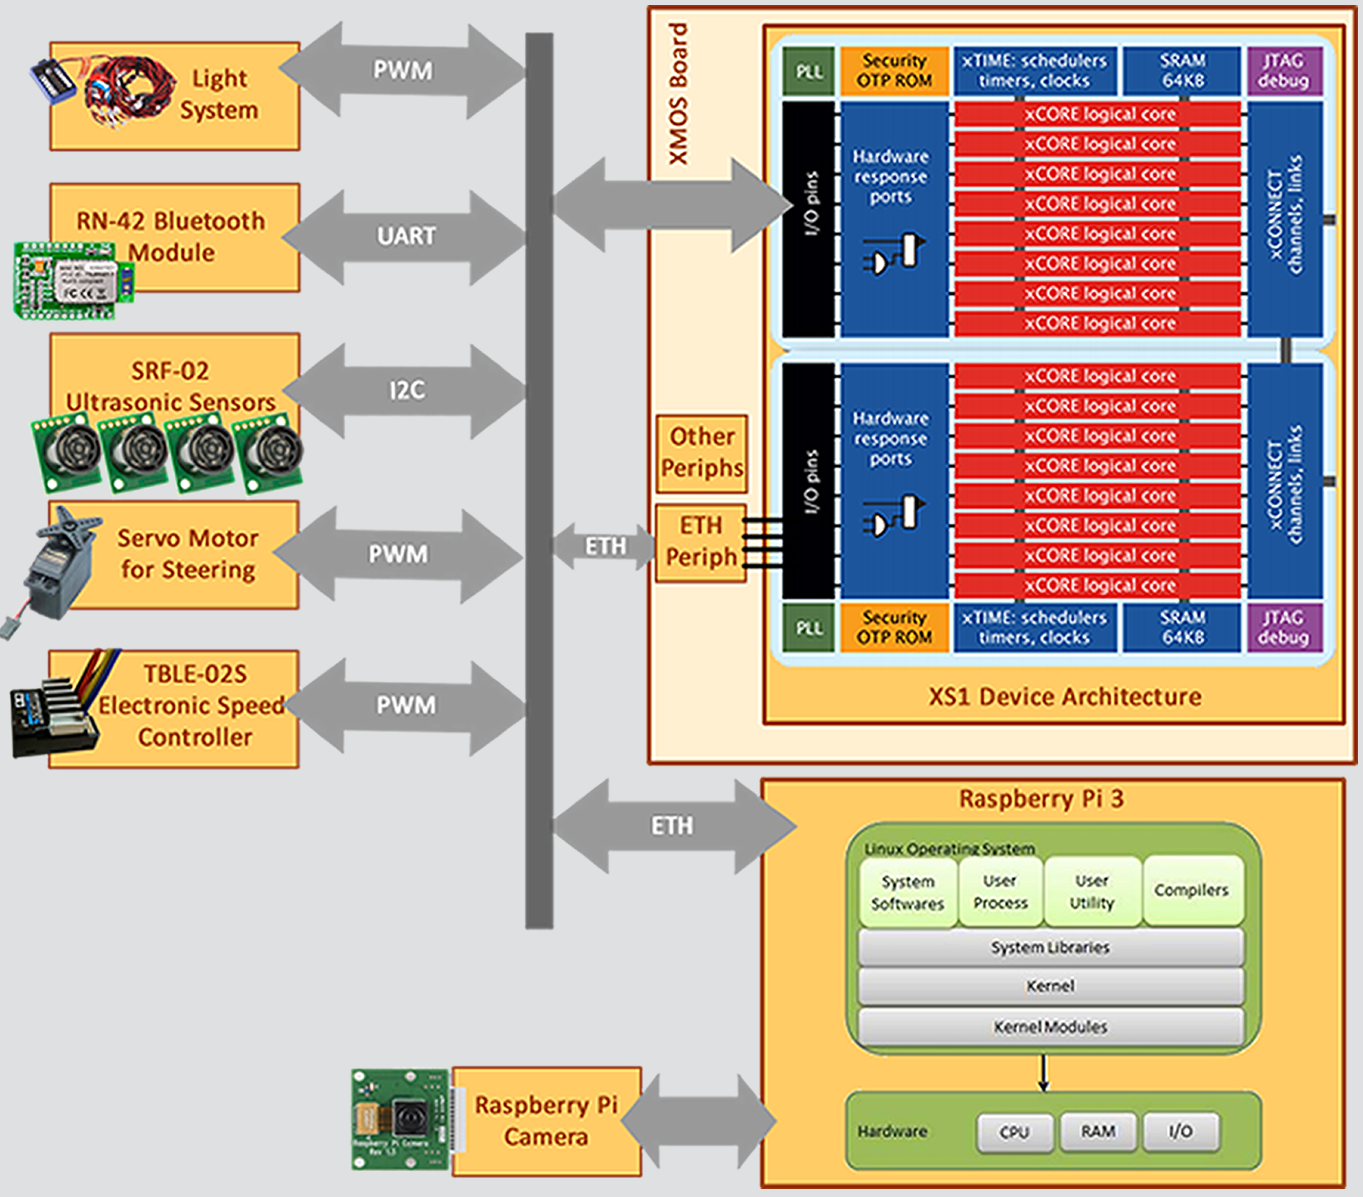
\includegraphics[scale=0.15]{images/hwarch.png}
	\caption{\label{Fig_Magnet}Magnetization as a function of applied field. Note 
	how the caption is centered in the column.}
\end{figure}

%EQUATION-----------------------------------------------
%\begin{equation}
%\label{Eq_1}
%\lambda_i = \lim \frac{1}{p} \sum_{t=1}^p \ln \frac{|w_i (t)|}{|w_i (t-1)|}
%\end{equation}

\section{Precise modeling and Software Parallelization}
\label{sec:impl}

%FIGURE-----------------------------------------------
%\begin{figure}[bth]
%\centering
%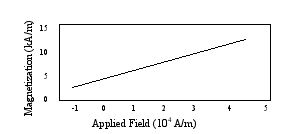
\includegraphics[scale=0.6]{images/Fig1.png}
%\caption{\label{Fig_Magnet}Magnetization as a function of applied field. Note 
%how the caption is centered in the column.}
%\end{figure}

%TABLE-----------------------------------------------
%\begin{table}[htb]
%\caption{Table Type Styles}
%\label{Table_I}1
%\centering
%\begin{tabular}{|p{1.2cm}|p{1.5cm}|p{1.5cm}|p{1.5cm}|}
%\hline
%\multirow{2}{1.2cm}{\textbf{Type Size (pts.)}} & \multicolumn{3}{|c|}{\textbf{Appearance}}\\
%\cline{2-4}
% & \textbf{\textit{Regular}}&\textbf{\textit{Bold}}&\textbf{\textit{Italic}}\\
%\hline
%8 & References, table header, footnotes, text subscripts, and superscripts &&\\
%\hline
%\end{tabular}
%\end{table}

\section{Evaluation and Related Work}
\label{sec:eval}

\section{Conclusion}
\label{sec:concl}

\section*{Acknowledgment}
The authors would like to express their appreciation to ...
\enlargethispage{-7in}

\bibliographystyle{IEEEtran}
\bibliography{ref}
\end{document}